\documentclass[problem]{mcs}

\begin{pcomments}
  \pcomment{FP_network_probability}
  \pcomment{from: F08.final}
\end{pcomments}


\pkeywords{
  congestion
  probability
  network
  routing}

%%%%%%%%%%%%%%%%%%%%%%%%%%%%%%%%%%%%%%%%%%%%%%%%%%%%%%%%%%%%%%%%%%%%%
% Problem starts here
%%%%%%%%%%%%%%%%%%%%%%%%%%%%%%%%%%%%%%%%%%%%%%%%%%%%%%%%%%%%%%%%%%%%%


\begin{problem} % \label{network} \ptitle{Packet Racket!}

  Consider the complete ternary-tree network with 9 inputs and 9 outputs
  shown below where packets are routed randomly.  The route each packet
  takes is the shortest path between input and output.  Let $I_0$, $I_1$,
  and $I_2$ be indicator random variables for the events that a packet
  originating at $in_0$, $in_1$, and $in_2$, respectively, crosses the
  dashed edge in the figure.  Let $T=I_0+I_1+I_2$ be a random variable for
  the number of packets passing through the dashed edge.

\vspace{12pt}
\centerline{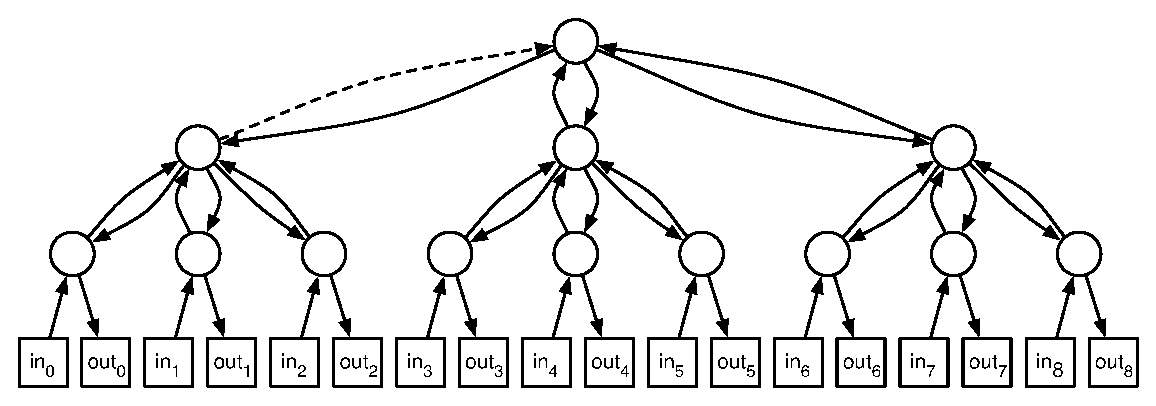
\includegraphics[width=6.5in]{ternary-network}}
\vspace{12pt}

\bparts

% \ppart{??} What is the diameter of this network, including the edges
% connected to the inputs and outputs?
%
% \solution[\vspace{0.5in}]{The diameter is the length of the shortest
%   distance between the input and output that are farthest apart. Any
%   path that goes through the top node is a longest path (for example
%   that from $\mathrm{in_0}$ to $\mathrm{out_8}$) with length 6.}

\ppart \label{edgepacketprob} %10

Suppose that each input sends a single packet to an output selected
uniformly at random; the packet destinations are mutually
independent. (Note that outputs may receive packets from multiple inputs
including their corresponding input.)

What are the expectation and variance of $T$?

\examspace[1in]

\begin{solution}
  A packet will pass through the dashed edge if it originates in inputs
  0--2 and is destined for outputs 3--8.  For $j \in \{0,1,2\}$ Let $I_j$
  be an indicator random variable for the event that a packet leaving
  input $j$ passes through the dashed edge.  The probability of this event
  is $\frac{2}{3}$. It follows that:

\begin{align*}
T & = I_1 + I_2 + I_3 \\
Ex[T] 
&= Ex[I_1 + I_2 + I_3] \\
&= Ex[I_1] + Ex[I_2] + Ex[I_3] \\
&= 3\cdot\frac{2}{3} \\
&= 2
\end{align*}

Similarly, by the linearity of variance for independent random variables:

\begin{align*}
T & = I_1 + I_2 + I_3 \\
Var[T] 
&= Var[I_1 + I_2 + I_3] \\
&= Var[I_1] + Var[I_2] + Var[I_3] \\
&= 3 \cdot \frac{2}{3} \cdot \left(1-\frac{2}{3}\right) \\
&= \frac{2}{3}
\end{align*}

\end{solution}

\ppart%{5}

Now consider the situation where a permutation of inputs to outputs is
chosen uniformly at random; each input sends a packet to a distinct
output.

\textbf{Old version:} What is the expected value of $T$?  Briefly justify your answer.

\textbf{New version:} Briefly explain why the expected value of $T$ is the
same as part~\eqref{edgepacketprob}, but the variance is not.  [Maybe ask
for the variance?]

\examspace[1in]

\begin{solution}
  Part~\eqref{edgepacketprob} expectation only used linearity and
  $\pr{I_i}=2/3$, which still holds, it still applies.  However, the
  indicators $I_1,I_2,I_3$ are not pairwise independent, so the variance
  argument does not hold.

\end{solution}

\eparts
\end{problem}

%%%%%%%%%%%%%%%%%%%%%%%%%%%%%%%%%%%%%%%%%%%%%%%%%%%%%%%%%%%%%%%%%%%%%
% Problem ends here
%%%%%%%%%%%%%%%%%%%%%%%%%%%%%%%%%%%%%%%%%%%%%%%%%%%%%%%%%%%%%%%%%%%%%

\endinput
